\chapter{Alloy Specification Framework}\label{c:alloy}

As aforementioned, this thesis aims to tackle the security vulnerabilities resulted from the miss-configuration over ROS files. In this chapter, it is intended to explore the Alloy framework that is relevant to overcome the above-mentioned challenge. % as well as previous developed work that has the same or similar goals as this thesis (\ref{s:alloy-relWork}).

The increasingly usage of robotics onto safety-critical systems results in demanding considerations over ensuring the proper correctness of both software and hardware, as failures mainly regarding the security domain might lead to fatal consequences. Thus, the use of formal methods and verification techniques, especially in systems highly reliant on flexibility and reliability, is recommended to avoid security-critical faults. \cite{carvalho2020analysis, clarke2011model} Software frameworks designed for this purpose must provide methods to perform structural design over systems with rich structures, abstracting their behaviour as a conventional model. Additionally, these frameworks must support features to enable automate analysis, in which property evaluation over these designed models is used as technique. 

The \textit{Alloy Framework} \cite{alloy-DJ}, fits within within this context, as it furnishes a declarative relation-based language, used for software modelling, complemented with extended tools supporting analysis over these models. \cite{alloy-6} The language combination of both relational and linear temporal logic (LTL) enables the ability to model both systems with rich structures and complex behaviour. To address the correctness over the specified model, Alloy performs model-checking techniques over these logic languages, where the model $M$ is exhaustively checked over property verification. \cite{lwspecification, carvalho2020analysis}

The framework \textit{analyzer} takes the specified model's restrictions into account, performing bounded and unbounded model checking to find instances that satisfy those implied restrictions. It can be also be useful for checking model properties, where the analyzer will try to return a counterexample instance. Instances are displayed by the framework Visualizer, alongside with the modelling process steps, regarding a trace representation. Instances appearance can be customized, using the \textit{theme}'s extension. \cite{alloy-6}

This chapter will go through these principles in further depth, to give the reader a proper review on how Alloy is structured, as its importance as a model checker to the computation domain, supported by a previously configured example where ROS communication architecture is structurally modelled. Since system analysis rely on the reasonable implementation of Model-Checking techniques, the follwing section within this subject intends to cover a clear contextualization on this matter. % since it is highly important on understanding how Alloy's verification process works.

\section{Model Checking}

% Model-checking is increasingly popular in the early phases of the software development process. To establish the cor- rectness of a software design one must usually verify both structural and behavioral (or temporal) properties. Unfor- tunately, most specification languages, and accompanying model-checkers, excel only in analyzing either one or the other kind. This limits their ability to verify dynamic systems with rich configurations: systems whose state space is character- ized by rich structural properties, but whose evolution is also expected to satisfy certain temporal properties. To address this problem, we first propose Electrum, an extension of the Alloy specification language with temporal logic operators, where both rich configurations and expressive temporal properties can easily be defined. Two alternative model-checking techniques are then proposed, one bounded and the other unbounded, to verify systems expressed in this language, namely to verify that every desirable temporal property holds for every possible configuration.

Performing software testing has been regarded as the established assessment procedure in which functional and non-functional specifications are evaluated. The conventional approach on software verification is based on testing the system with different inputs, to achieve quality assurance over several intended specifications. \cite{beyer2017software, briand2001uml} As this technique demands exhaustively evaluation over pre-selected test data, it is commonly explored over automated tools, since manual testing is time-consuming and prone to errors. \cite{clarke1976program, fraser2009testing} 

% Model-based testing arises as a viable alternative technique, in which both test cases and intended behaviour relies on the design of an abstract mode, presenting remarkable benefits to the latter approach. \cite{apfelbaum1997model} Thus, to perform full verification over systems, the \textit{model-checking} technique can be used to automatically interpret counterexamples as test cases, consequently enabling far better degrees of coverage than conventional testing. \cite{fraser2009testing, beyer2017software}

\textit{Model Checking} presents itself as a novel technique with the purpose of verifying temporal properties over the system finite-state that is duly represented as a conclusive model. Additionally, it enables \textit{model-based testing} by automatically interpreting counterexamples as test cases, resulting in significantly greater degrees of coverage than conventional testing. \cite{fraser2009testing, beyer2017software} This technique is becoming highly used due to its importance as an early phase approach upon developing systems \cite{lwspecification}, as it confers the most valued functionality over model-checkers, which concrete models, regarding the software architecture, is exhaustively checked over behavioral properties. 

It provides highly automatic verification procedures, in which other techniques, such as theorem provers fails to address, due to its deductive reasoning nature. The representation of not satisfied specifications over counterexamples, confers great functionality to this technique, often required for debugging matters.
However, the system's inevitable state expansion consequently causes the complexity increase on verification procedure. This is referred to as the \textit{state explosion problem}, in which model-checking is unable to handle the size of the state space, failing as system verifying technique. \cite{clarke2011model, clarke1997model} 

% Bounded e Unbounded techniques ? Alloy accounts both techniques ....
\subsection{Bounded Model Checking}

\subsection{LTL Model Checking}

\section{Structural Design}

The \textit{Alloy framework} presents itself as a formal modelling language, conceived to properly address model-checking techniques over their specification language, where both structural design and temporal behaviour, naturally specified over properties, can easily be defined. Formerly, Alloy was inherently static \cite{lwspecification}, meaning that it only excel the structural design, where its language was based on first-order logic. The analysis process relied on a bounded model checking technique with no support for temporal behaviour. Notwithstanding, the latest realease of Alloy confers the ability to properly deal with expressive temporal properties, as well as trace evaluation over time, while employing the former structural approach. 

As intentionally design to formally abstract both system's configuration and behaviour, Alloy successfully incorporates a set of features, within a well-documented and wide-ranged syntax that consequently allows large specification development. \cite{carvalho2020analysis} The following subsection \ref{c:alloy-sm} addresses the Alloy concepts required for understanding how system modelling is covered. 

% Before accurately accounting both structural design as modelling technique and structural analysis, it follows the Alloy formal syntax.

\newpage 

\begin{lstlisting}[title={Alloy's syntax.}]
alloyModule ::= [moduleDecl] import* paragraph*
moduleDecl ::= module qualName [[name,+]]
import ::= open qualName [[qualName,+]] [as name]
paragraph ::= sigDecl | factDecl | predDecl | funDecl
    | assertDecl | cmdDecl
sigDecl ::= [var] [abstract] [mult] sig name,+ [sigExt] { fieldDecl,* } [block]
sigExt ::= extends qualName | in qualName [+ qualName]*
mult ::= lone | some | one
fieldDecl ::= [var] decl
decl ::= [disj] name,+ : [disj] expr
factDecl ::= fact [name] block
predDecl ::= pred [qualName .] name [paraDecls] block
funDecl ::= fun [qualName .] name [paraDecls] : expr { expr }
paraDecls ::= ( decl,* ) | [ decl,* ]
assertDecl ::= assert [name] block
cmdDecl ::= [name :] ( run | check ) ( qualName | block ) [scope]
scope ::= for number [but typescope,+] | for typescope,+
typescope ::= [exactly] number qualName
expr ::= const | qualName | @name | this
    | unOp expr | expr binOp expr | expr arrowOp expr
    | expr [ expr,* ]
    | expr [! | not] compareOp expr
    | expr ( => | implies ) expr else expr
    | let letDecl,+ blockOrBar
    | quant decl,+ blockOrBar
    | { decl,+ blockOrBar }
    | expr '
    | ( expr ) | block
const ::= [-] number | none | univ | iden
unOp ::= ! | not | no | mult | set | # | ~ | * | ^ 
    | always | eventually | after | before | historically | once
binOp ::= || | or | && | and | <=> | iff | => | implies | 
    & | + | - | ++ | <: | :> | . | until | releases | since | triggered | ;
arrowOp ::= [mult | set] -> [mult | set]
compareOp ::= in | = | < | > | =< | =>
letDecl ::= name = expr
block ::= { expr* }
blockOrBar ::= block | bar expr
bar ::= |
quant ::= all | no | sum | mult
qualName ::= [this/] ( name / )* name
\end{lstlisting}

\newpage

\subsection{System Modelling}\label{c:alloy-sm}

Alloy aims to address the complexity behind richly structured systems, that require critical control over their intended behaviour, by presenting a novel approach for abstracting these systems as conventional models. System's structures can be specified over time-evolving states, where its behaviour clearly identifies the states' inbetween transitions. Thus, the conception of system transitioning offers a great formal approach when it comes to reason about the system's design.

The Alloy structural definition relies on a relation way of connecting system's elements, where the latter is abstracted in terms of relations. In Alloy, unary relations, commonly known as sets, are labelled as \textit{signatures}, that are inhabited by a set of \textit{atoms}, from a finite universe of discourse. Atoms are perceived as the lowest-grain elements, with no particular semantics attached. A signature, identified by the keyword \textit{sig}, might include multiple \textit{field} declarations enclosed between braces, addressing relation between the signature's atoms and a set or other relation. Fields are inhabited by tuples of atoms from the universe, that must meet the same arity.

Signatures can either be perceived as a top-level signature, or as other signature's subset. Signature hierarchy is conceivable through disjoint extensions (\textit{extends}), or by set inclusion (\textit{in}). The \textit{abstract} keyword declares a signature that contains no atoms beyond those within its extensions. 

To address default configuration over the universe's multiplicity, both signatures and fields can be specified under a multiplicity constraint. The former constrains the number of signature atoms, where it is commonly used to express singleton sets, over the constraint keyword \textit{one sig}. Fields, however, makes great use of multiplicities, offering behaviour expressness over relations between atoms. Additionally to these model constraints, implicitly specified over the course of the modelling process, system assumptions can be defined over axioms, expressed as \textit{facts}, where multiple constraints can be incorporated.

Moreover, the lattest Alloy version enables evaluation changing throughout the trace evolution, consequently allowing the consideration of both signatures and fields as time mutable declarations, through the usage of the keyword \textit{var}.

Throughout the sections that follow, it will be presented an illustrive example over which graph theory rests, this being the study of \textit{Eulerian Circuits}. This example will be used to duly contextualize both modelling and verification process in Alloy. \textit{Eulerian Circuits} must meet several behaviour constraints over the classic graph definition, that must be addressed over axioms. However, the structural modelling must be provided beforehand.

\subsubsection{Model Structure}

The \textit{Eulerian} path denotes a trail within a finite graph, with each graph edge being visited precisely once. Thus, this already implies that the graph must be connected, where each node must be reachable, and undirected, where edges are non-oriented. 

\begin{lstlisting}[title={Graph definition.}, otherkeywords = {abstract, sig, module, set, fact, iden, no, in}]
module graph

abstract sig Node {
    adj : set Node
}

fact considerations {
    adj = ~adj
    no iden & adj
    Node->Node in *(adj + ~adj)
}
\end{lstlisting}


% Everything is a relation

\subsection{System Behaviour}

Model's behaviour representation represents the ability to express what is intended to happen during state transitions over the valid traces of a system. A \textit{trace} is represented as an infinite chain of states that completely describes a system's potential behavior.

Valid traces are constrained by explicit specification of axioms, identified using the \textit{facts} keyword. However, as explained above, model assumptions covered by each \textit{signature} declaration, also constrains the system's behaviour. 


\subsubsection{Behaviour Representation}

% As previously explained, the model assumptions that are not covered by the signatures structure, should be declared within Electrum facts. However, not every property that we’re interested in validating and reason about, should be an assumption. Predicates are reusable boolean formulas built through Electrum expressions. All of these features, as well as the notion of reusable expressions (fun) and model assertions (assert), are conceptually grouped into Electrum paragraphs, as shown in the formal syntax 

\section{Structural Analysis}

Structural modelling only confers an conventional way of formally expressing the intended behaviour over a software component. To perform verification over the specified behaviour, it is advisable to implement analysis techniques, while supporting a illustrative way of exploring the behaviour through simulations. 

This section aims to explain how Alloy conducts system analysis, with further explanations over the corresponding analysis commands, along with an overview on the Alloy Analyzer interactive exploration over a system's design. 

\subsection{System Analysis and Verification}

Alloy specification process does not establish a clear process separation over the model design and model analysis. This implies that analysis over model checking also accounts the model itself as a combination of properties specification. 

The specification language holds \textit{two} analyzing commands, \textit{run} and \textit{check} respectivaly, as shown above in \textit{Alloy's syntax}. A \textit{Linear Temporal Logic (LTL) formula} is enclosed between braces, to be checked over. Upon executing, both commands accounts the enclosed formula $\psi_{f}$, as well as the model declaration ${M}$. Likewise in \textit{facts} declaration, several logic constraints can be combined into the formula $\psi_{f}$. Due to Alloy's implicit abstraction, both commands addresses the relational model specification as truth holder, with the latter being consisted by declarations over \textit{facts} and \textit{signatures}. 

Briefly speaking, \textit{run} instruct the model-checker to present an example that satisfies the considered formula $\psi_{f}$ over the model definition. This means that the following formula ($M \wedge \psi_{f}$) is expected to hold. The consistency of the \textit{facts} and \textit{signatures} is consequently verified since the model declaration $M$ is also considered in the latter formula. 

Alloy makes use of the \textit{check} command to perform automatic verification over an \textit{assertion} declaration. The assertion $\psi_{f}$ verification is done over proving if the following satisfiability formula $M \models \psi_{f}$ is valid within the defined scopes. % while it accounts the declared \textit{facts} as truth holders. 

As result of the first-order logic's undecidability problem, the consistency proofness over satisfiability formulas is not possible. \cite{vakili2012temporal} To ensure decidability, the Alloy Analyzer performs analysis over \textit{scopes}, assigned to each signature declaration. By default, if no scope is provided, the model-checker will account at most \textit{three} atoms for each signature, upon trying to provide an \textit{instance} that satisfies the former formula, consequently proving the behaviour specification (\textit{facts} considerations) consistency. Also, as scopes imposes a limit on the state space of an Alloy model, if no \textit{run} instance is returned, the formula can not be perceived as inconsistent, as scopes can not be properly set to satisfy the latter.

\begin{figure}[H]
    \centering
    
\includegraphics[width=0.4\linewidth]{images/check_alloy_1.png}
    \caption{LTL formula $\psi$ verification using \textit{check}, accounting the \textit{Bounded} model checking technique.}
    \label{fig:alloy-check-1}
\end{figure}

Being SAT-based \cite{lwspecification}, the Alloy Analyzer tries to search for a \textit{lasso trace} instance that satistfies the formula $M \models \psi_{f}$ over the \textit{check} command, it performs the latter refutation ($(M \wedge \neg \psi_{p})$ by applying \textit{De Morgan's laws}), yielding a counter-example if the latter is satisfied. This technique is called \textit{Proof by Refutation}: $M$ entails $\psi_{p}$, denoted by $M \models \psi_{f}$, \textit{if and only if} $(M \wedge \neg \psi_{p})$ is unsatisfiable, reducing validity to unsatisfiability.

\begin{figure}[H]
    \centering
    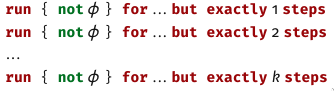
\includegraphics[width=0.5\linewidth]{images/check_alloy_2.png}
    \caption{Reducing Validity to Unsatisfiability.}
    \label{fig:alloy-check-2}
\end{figure}

Moreover, Alloy yields a command to specify the finite number of different steps, related to the expected intance's evaluation trace. This is due to the \textit{bounded} nature of the Alloy transitions between states, where the \textit{Bounded Model Checking} technique is considered as model-checking technique. The number of steps is set to \textit{ten} by default, although this may be adjusted using the keyword \textit{steps}, alonside with the bounded scopes specification. 

\subsubsection{Relevant Properties}

The verification process over \textit{Model Checking}, needs to account the formal specification of properties that are relevant to reason about the system's behaviour. \cite{baier2008principles} With regard of ensuring the correctness of a system's expected behaviour, \textit{Safety} and \textit{Liveness} properties must be appropriatly specified, where its verification technique was motivated by distinct techniques. \cite{kindler1994safety} The former requires an invariance argument, where the latter requires a well-foundedness argument to prove its system satisfiability. \cite{alpern1987recognizing}

A \textit{safety property} asserts that "nothing bad should happen" during the system execution, meaning that, every trace state is expected. Consequently, if a trace that jeoperdizes a safety property is found, it can be assumed that the latter has a "bad" property prefix. Whereas, a \textit{liveness property} expresses that "something good will happen", implying the eventual occurrence of a state during the course of the system's execution. \cite{lamport1977proving}

% Fairness Properties


\subsection{Alloy Analyzer}

The specification process is usually performed interactively. The user takes a first approach to the model specification, and then proceed to its refinement towards the model validation. In order to ease this process and improve the user comprehension of model instances and counter-examples, the Electrum Analyzer provides a Visualizer capable of showing a navi- gable set of graphical instances that are produced by command executions. A set of features that allow a full instance theme customization and an instant expression evaluation are also provided by the Analyzer.

% Model checking alloy e grafico kodkod etc
% alloy visualizer
% safety e liveness e fairness